\chead{CHAPITRE 4. SPRINT 2: Gestion de Recrutement et Candidatures}

\chapter{Sprint 2: Gestion de Recrutement et Candidatures}
\renewcommand{\mtctitle}{Sommaire}
\minitoc
	\newpage
\section*{Introduction}
Ce chapitre explore les étapes de la Sprint Gestion de Recrutement et Candidatures, avec un accent particulier sur la gestion des offres d’emploi et le processus de candidature. Nous débuterons par un aperçu du backlog, avant de détailler la conception, la mise en œuvre et d’illustrer le travail effectué à l’aide de captures d’écran.
\addcontentsline{toc}{section}{\protect\numberline{}Introduction}%
\section{Objectifs du Sprint}
L’objectif de cette sprint est de permettre la gestion des offres d’emploi par le responsable RH, ainsi que de faciliter la consultation et la soumission de candidatures par les candidats.

\section{Spécification des besoins}
\par Dans cette section, nous allons débuter par présenter le diagramme de cas d’utilisation de la sprint, suivi de l’exposition du backlog associé.
\subsection{Diagramme cas d’utilisation du Sprint 2}


\begin{figure}[H]
\centering
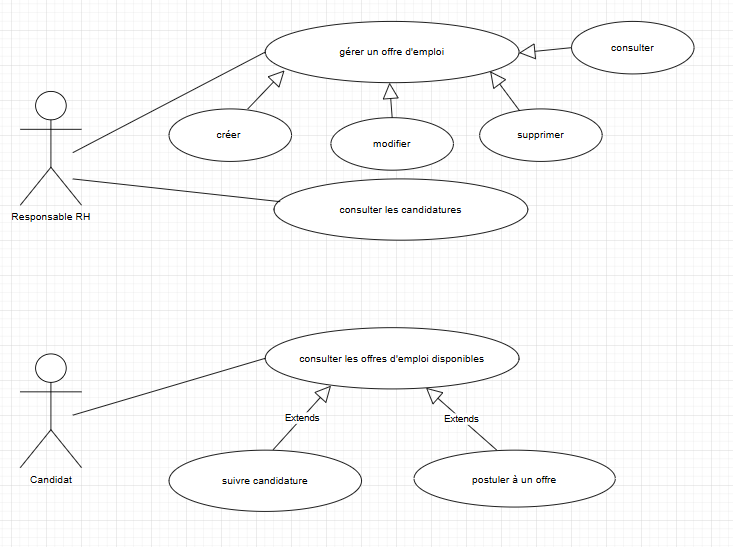
\includegraphics[width=14cm, height=11cm]{Figures/use case 2.png}
\caption{Diagramme cas d’utilisation du sprint 2}
\label{schema1}
\end{figure}
 
\subsection{ Sprint backlog du sprint 2}
Le tableau ci-dessous présente le sprint backlog établi pour le deuxième sprint. Il récapitule les différentes user stories sélectionnées, accompagnées de leurs identifiants uniques, ainsi que les tâches techniques à réaliser pour chacune. Ce tableau permet d’avoir une vision claire et structurée du travail prévu, en facilitant la planification, la répartition des responsabilités et le suivi de l’avancement tout au long du sprint.
\begin{table}[H]
\caption{Backlog du sprint 2}
\centering
\begin{tabular}{|p{1cm}|p{8cm}|p{8cm}|}
\hline
\textbf{ID} & \textbf{User Story} & \textbf{Tâches techniques} \\
\hline
US-8 & En tant que responsable RH, je veux créer, modifier et consulter des offres d’emploi afin d’attirer des candidats. 
& 
\begin{itemize}[leftmargin=*]
  \item Créer le modèle "Offre d'emploi".
  \item Développer le formulaire de création/modification.
  \item Implémenter les vues CRUD.
  \item Connecter à la base de données.
\end{itemize} \\
\hline
US-9 & En tant que candidat, je veux consulter toutes les offres d’emploi disponibles. 
& 
\begin{itemize}[leftmargin=*]
  \item Créer une page d'affichage des offres.
  \item Développer une API pour lister les offres.
  \item Mettre en place un filtre de recherche.
\end{itemize} \\
\hline
US-10 & En tant que candidat, je veux postuler à une offre d’emploi. 
& 
\begin{itemize}[leftmargin=*]
  \item Créer le modèle de "Candidature".
  \item Implémenter le bouton de candidature.
  \item Enregistrer la candidature dans la base.
\end{itemize} \\
\hline
US-11 & En tant que candidat, je veux suivre l’état de mes candidatures. 
& 
\begin{itemize}[leftmargin=*]
  \item Créer une vue "Mes candidatures".
  \item Ajouter un champ "état" (en cours, accepté, refusé).
\end{itemize} \\
\hline
US-12 & En tant que responsable RH, je veux accéder à la liste des candidatures. 
& 
\begin{itemize}[leftmargin=*]
  \item Créer la vue "Liste des candidatures".
  \item Créer un filtre de recherche.
  \item Lier avec le backend des candidatures.
\end{itemize} \\
\hline
\end{tabular}
\label{tab:sprint2_backlog}
\end{table}

\section{Analyse des besoins}
Avant de modéliser les fonctionnalités du système, il est essentiel de comprendre les besoins fonctionnels exprimés à travers les différents cas d’usage. La section suivante propose une description textuelle de ces cas d’utilisation, permettant de mieux cerner les interactions entre les utilisateurs et le système, et de poser les bases d’une modélisation cohérente.
    
\subsection{Description textuelle de cas d'utilisation}
    \begin{itemize}
        \item \textbf{Cas d'utilisation "Gérer une offre d'emploi": } La table 4.2 ci-dessous présente la description textuelle du cas d'utilisation « Gérer une offre d'emploi ».
    \end{itemize}
    \begin{table}[H]
    \caption{ Description textuelle du cas d’utilisation "Gérer une offre d'emploi"}
    \centering
    \begin{tabular}{|c|p{12cm}|}
    \hline
    \textbf{Titre} & Gérer une offre d'emploi \\
    \hline
    \textbf{Objectif} & Permettre au responsable RH de gérer les offres d’emploi (création, modification, archivage). \\
    \hline
    \textbf{Acteur}& Responsable RH\\
    \hline
    \textbf{Pré-condition} & Le responsable RH doit être authentifié et avoir les droits d’accès nécessaires.
    \\
    \hline
    \textbf{Post-condition} & Les modifications ou archivages des offres sont enregistrés dans le système.\\
    \hline
    \textbf{Scénario nominal} & 1. Le responsable RH accède à l’interface de gestion des offres. \newline
    2. Il sélectionne une action (créer, modifier, archiver).\newline
    3. Il entre ou modifie les détails de l’offre (titre, description, etc.).
    \newline
    4. Le système valide et enregistre les changements.\\
    \hline
    \end{tabular}
    \label{tab:user_stories}
\end{table}

\begin{itemize}
        \item \textbf{Cas d'utilisation "Consulter les candidatures": } La table 4.3 ci-dessous présente la description textuelle du cas d'utilisation « Consulter les candidatures ».
    \end{itemize}
    \begin{table}[H]
    \caption{ Description textuelle du cas d’utilisation "consulter les candidatures"}
    \centering
    \begin{tabular}{|c|p{12cm}|}
    \hline
    \textbf{Titre} & Consulter les candidatures \\
    \hline
    \textbf{Objectif} & Permettre au responsable RH de visualiser la liste des candidatures reçues pour une offre. \\
    \hline
    \textbf{Acteur}& Responsable RH\\
    \hline
    \textbf{Pré-condition} & Une offre d’emploi doit exister et des candidatures doivent avoir été soumises.
    \\
    \hline
    \textbf{Post-condition} & La liste des candidatures est affichée avec les détails des candidats.\\
    \hline
    \textbf{Scénario nominal} & 1. Le responsable RH accède à la gestion des offres. \newline
    2. Il sélectionne une offre spécifique.\newline
    3. Le système affiche la liste des candidatures.
    \newline
    4. Il consulte les détails des candidatures.\\
    \hline
    \end{tabular}
    \label{tab:user_stories}
\end{table}

\begin{itemize}
        \item \textbf{Cas d'utilisation "Consulter les offres d'emploi": } La table 4.4 ci-dessous présente la description textuelle du cas d'utilisation « Consulter les offres d'emploi ».
    \end{itemize}
    \begin{table}[H]
    \caption{ Description textuelle du cas d’utilisation "Consulter les offres d'emploi"}
    \centering
    \begin{tabular}{|c|p{12cm}|}
    \hline
    \textbf{Titre} & Consulter les offres d'emploi \\
    \hline
    \textbf{Objectif} & Permettre au candidat de visualiser les offres d’emploi disponibles sur la plateforme. \\
    \hline
    \textbf{Acteur}& Candidat\\
    \hline
    \textbf{Pré-condition} & Le candidat doit avoir accès à la plateforme .
    \\
    \hline
    \textbf{Post-condition} & La liste des offres d’emploi est affichée au candidat.\\
    \hline
    \textbf{Scénario nominal} & 1. Le candidat accède à la section des offres. \newline
    2. Il navigue dans la liste des offres.\newline
    3. Le système affiche les détails de chaque offre.
    \newline
    4. Il consulte les informations.\\
    \hline
    \end{tabular}
    \label{tab:user_stories}
\end{table}

\begin{itemize}
        \item \textbf{Cas d'utilisation "Postuler à une offre": } La table 4.5 ci-dessous présente la description textuelle du cas d'utilisation « Postuler à une offre ».
    \end{itemize}
    \begin{table}[H]
    \caption{ Description textuelle du cas d’utilisation "Postuler à une offre"}
    \centering
    \begin{tabular}{|c|p{12cm}|}
    \hline
    \textbf{Titre} & Postuler à une offre \\
    \hline
    \textbf{Objectif} & Permettre au candidat de soumettre une candidature pour une offre d’emploi. \\
    \hline
    \textbf{Acteur}& Candidat\\
    \hline
    \textbf{Pré-condition} & Le candidat doit avoir un compte actif et une offre doit être disponible.
    \\
    \hline
    \textbf{Post-condition} & La candidature est envoyée et enregistrée dans le système avec le profil du candidat.\\
    \hline
    \textbf{Scénario nominal} & 1. Le candidat accède à une offre d’emploi.\newline
    2. Il clique sur l’option "Postuler".\newline
    3. Le système soumet automatiquement son profil comme candidature.
    \newline
    4. Le système confirme l’envoi de la candidature.\\
    \hline
    \end{tabular}
    \label{tab:user_stories}
\end{table}

\begin{itemize}
        \item \textbf{Cas d'utilisation "Suivre les candidatures": } La table 4.6 ci-dessous présente la description textuelle du cas d'utilisation « Suivre les candidatures ».
    \end{itemize}
    \begin{table}[H]
    \caption{ Description textuelle du cas d’utilisation "Suivre les candidatures"}
    \centering
    \begin{tabular}{|c|p{12cm}|}
    \hline
    \textbf{Titre} & Suivre les candidatures \\
    \hline
    \textbf{Objectif} & Permettre au candidat de suivre l’état de ses candidatures soumises. \\
    \hline
    \textbf{Acteur}& Candidat\\
    \hline
    \textbf{Pré-condition} & Le candidat doit avoir un compte actif, un profil complété et au moins une candidature soumise.
    \\
    \hline
    \textbf{Post-condition} & L’état des candidatures du candidat est affiché et mis à jour dans le système.\\
    \hline
    \textbf{Scénario nominal} & 1. Le candidat se connecte à l’application.\newline
    2. Il accède à la section de ses candidatures.\newline
    3. Le système affiche la liste de ses candidatures avec leur état (en attente, accepté, refusé).
    \newline
    4. Il consulte les détails de chaque candidature.\\
    \hline
    \end{tabular}
    \label{tab:user_stories}
\end{table}

\section{Conception}
\hspace{0.5cm}\textbf Dans cette section, nous discutons de la conception du deuxième sprint. nous Commençons par le diagramme de classes du sprint. Ensuite, nous examinons la modélisation de quelques diagrammes de séquences. 



   
\subsection{Diagrammes de séquences}
Dans le cadre de l’analyse dynamique du système, un diagramme de séquence a été réalisé pour chaque fonctionnalité clé développée lors des sprints. Le diagramme ci-dessous illustre spécifiquement le scénario du cas d'utilisation « Gérer un offre d'emploi », permettant de visualiser les interactions entre le responsable rh et le système lors de la création d’un nouvel offre d'emploi.
\subsubsection{ Diagramme de séquence au scénario : «Gérer un offre d'emploi»}
Cette figure illustre le déroulement du scénario associé à ce cas d'utilisation.
     \begin{figure}[H]
    \centering
   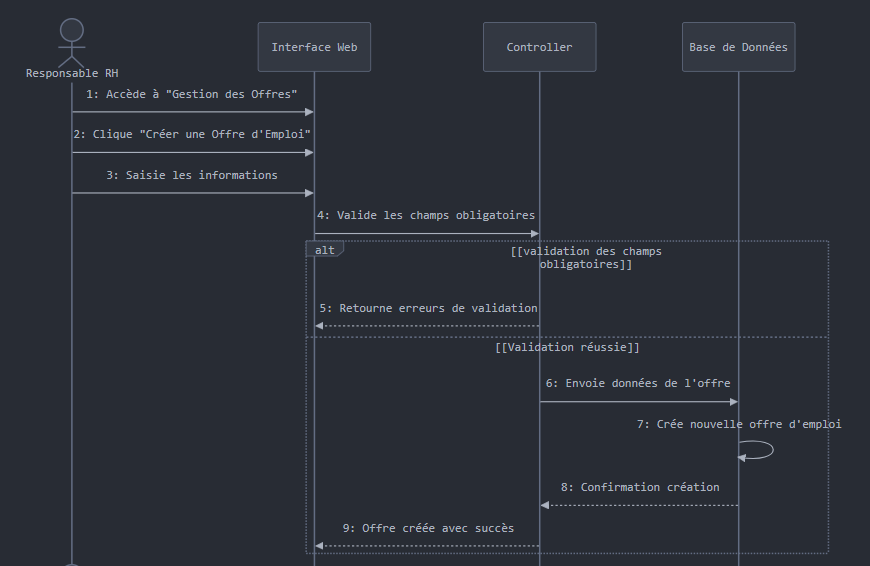
\includegraphics[width=18cm, height=18cm]{Figures/seq2.png}
    \caption{Diagramme de séquence détaillé au scénario «Gérer un offre d'emploi»}

\end{figure}
\section{Réalisation: interfaces utilisateur dans RhNova }
Dans cette partie, nous illustrons les principales interfaces conçues dans le cadre du processus de recrutement. Elles permettent aux responsables RH de gérer les offres et de suivre les candidatures, tandis que les candidats peuvent consulter les annonces disponibles et suivre l’état de leurs demandes.
\vspace{5mm}
\begin{itemize}
     \begin{itemize}
      \item \textbf{ Gestion des offres d'emploi : }Cette interface permet au responsable RH de créer, consulter et gérer les offres d’emploi. Il peut y renseigner les détails du poste (titre, département, type de contrat, lieu, salaire, date limite, etc.) ainsi que la description et les exigences du poste. Les offres actives est également visible et modifiable depuis cet espace.
         \begin{figure}[H]
             \centering
             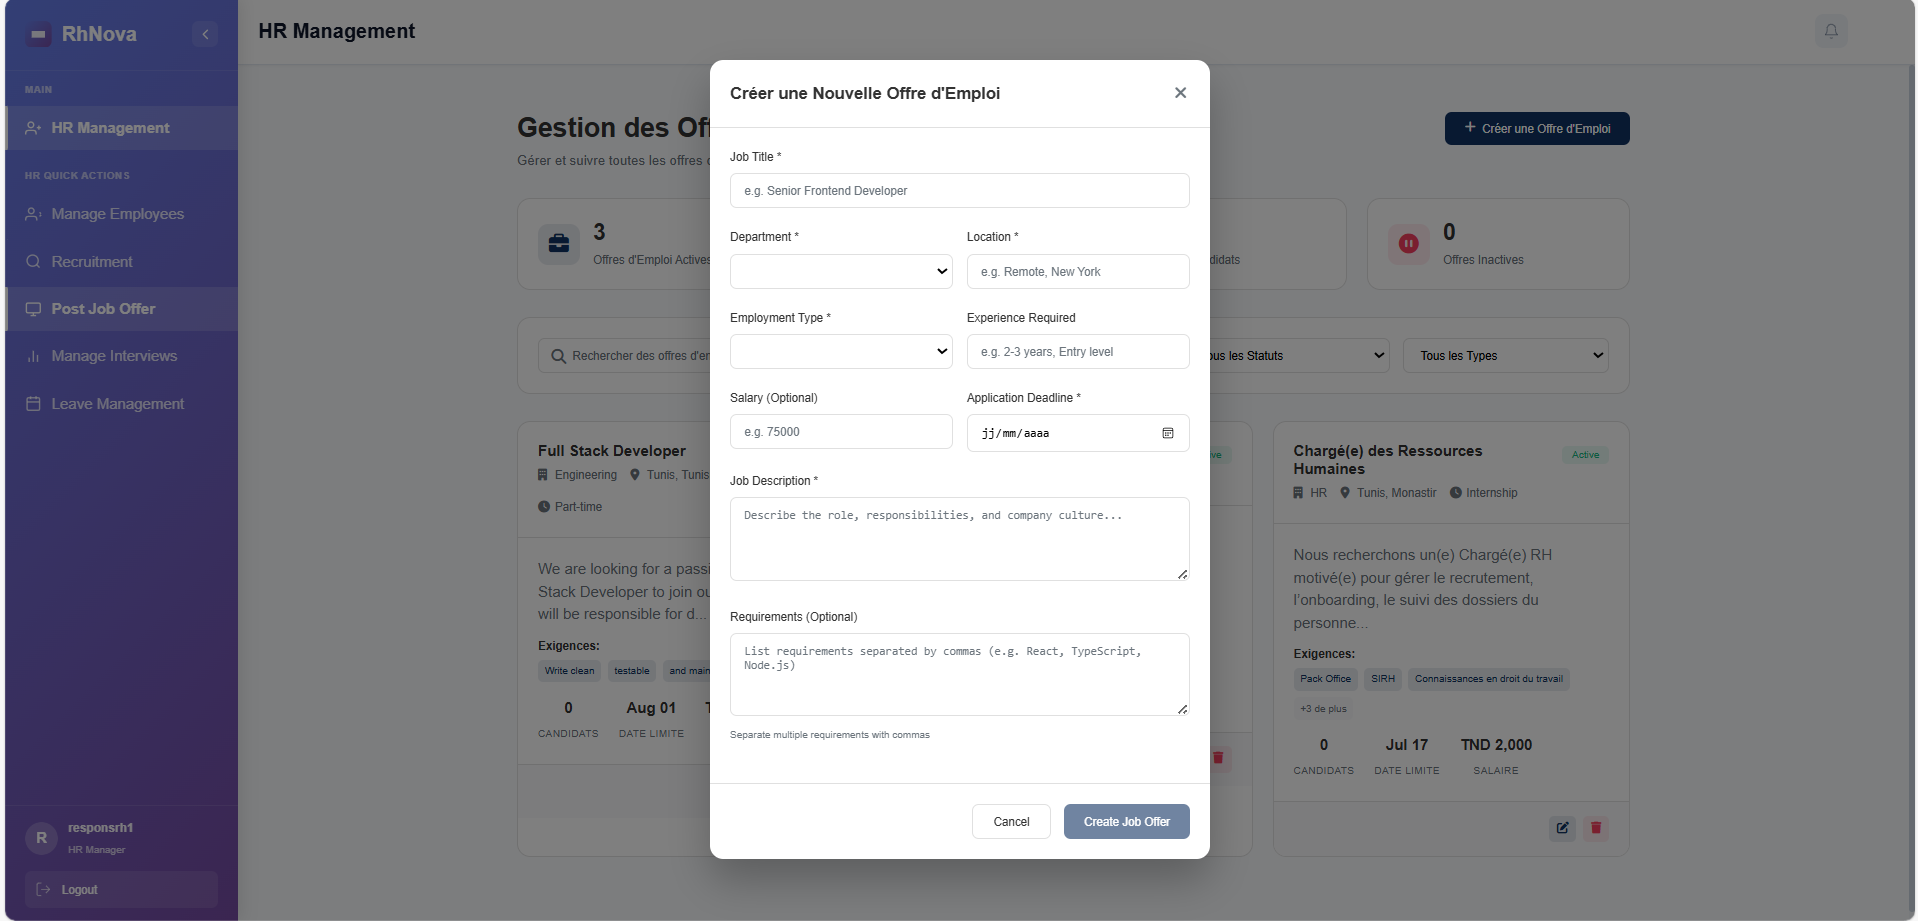
\includegraphics[width=\textwidth]{Figures/responsjoboffer.png}
             \caption{Page de gestion d'offre d'emploi}
         \end{figure}
     \end{itemize}
\end{itemize}
\begin{itemize}
     \item\textbf{Consultation des candidatures : }
Cette interface permet au responsable RH d'accéder aux candidatures reçues après filtrage automatique des CV par le système ATS. Il peut consulter les profils détaillés des candidats pour chaque offre, ce qui facilite l’évaluation et la présélection.
         \begin{figure}[H]
             \centering
             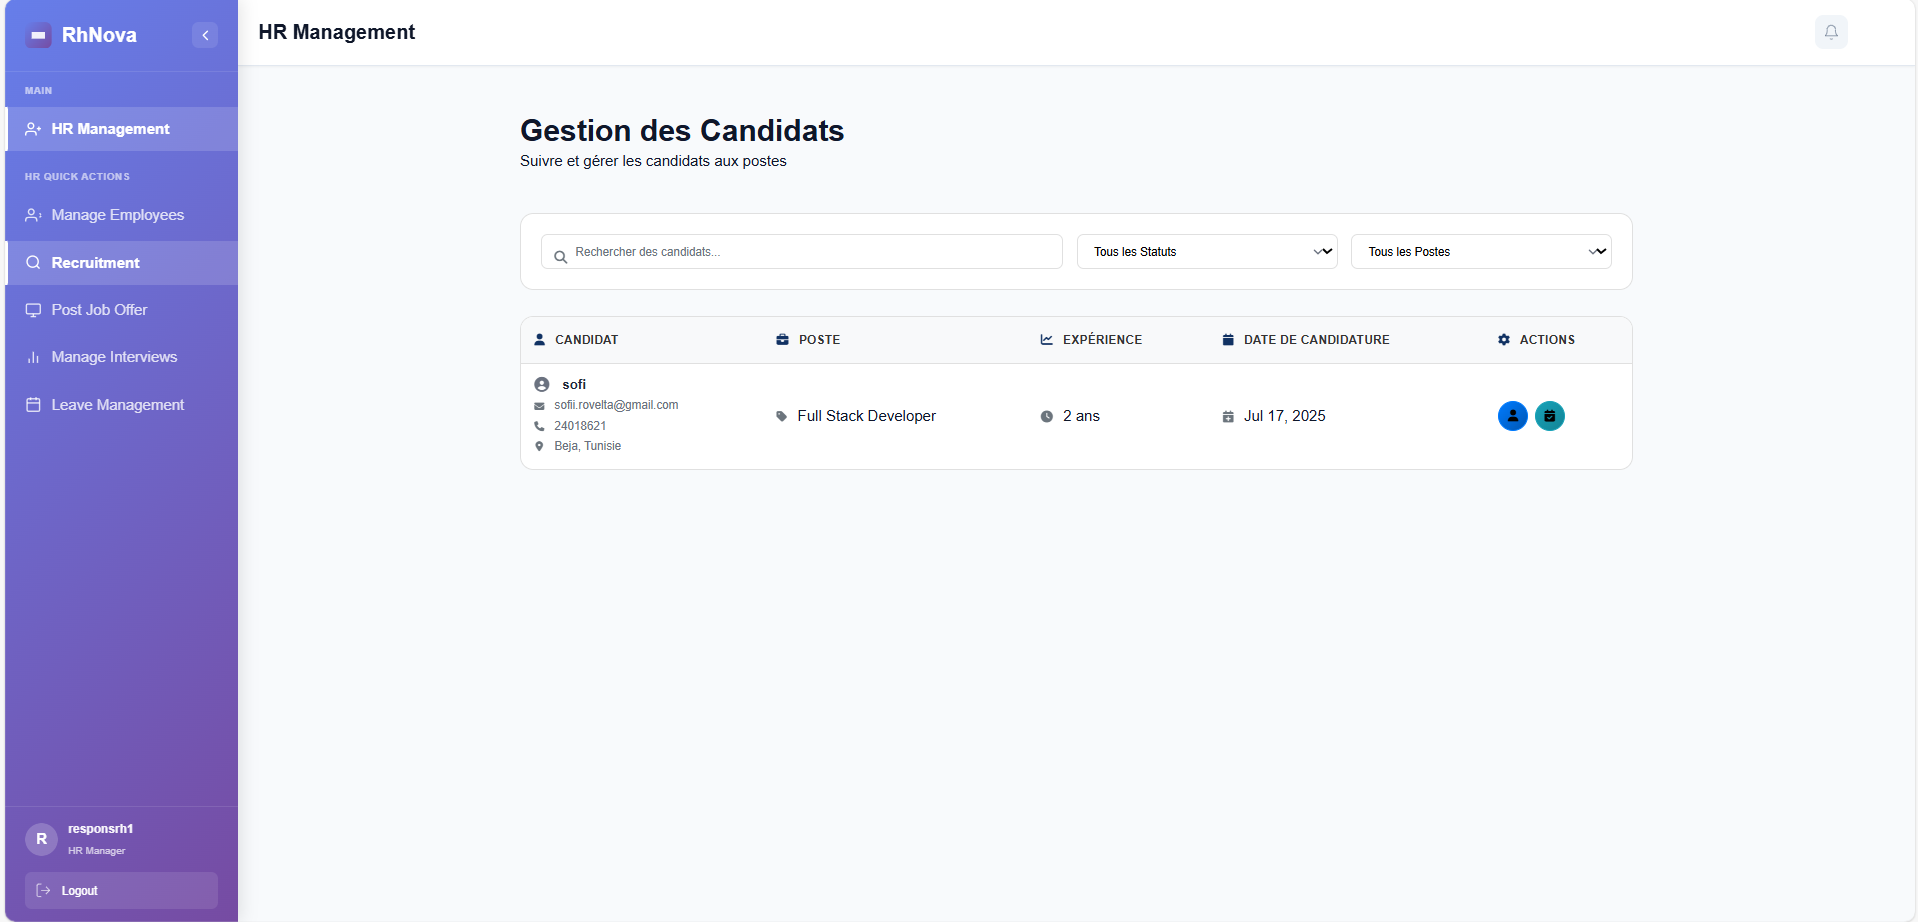
\includegraphics[width=\textwidth]{Figures/responscandidature.png}
             \caption{Liste des candidatures}
         \end{figure}
\end{itemize}
\begin{itemize}
     \item\textbf{Consultation des offres : }
Cette interface permet au candidat de consulter la liste des offres d’emploi disponibles avec leurs détails (poste, lieu, compétences, type de contrat). Il peut voir les informations complètes d’une offre et postuler directement en ligne.
         \begin{figure}[H]
             \centering
             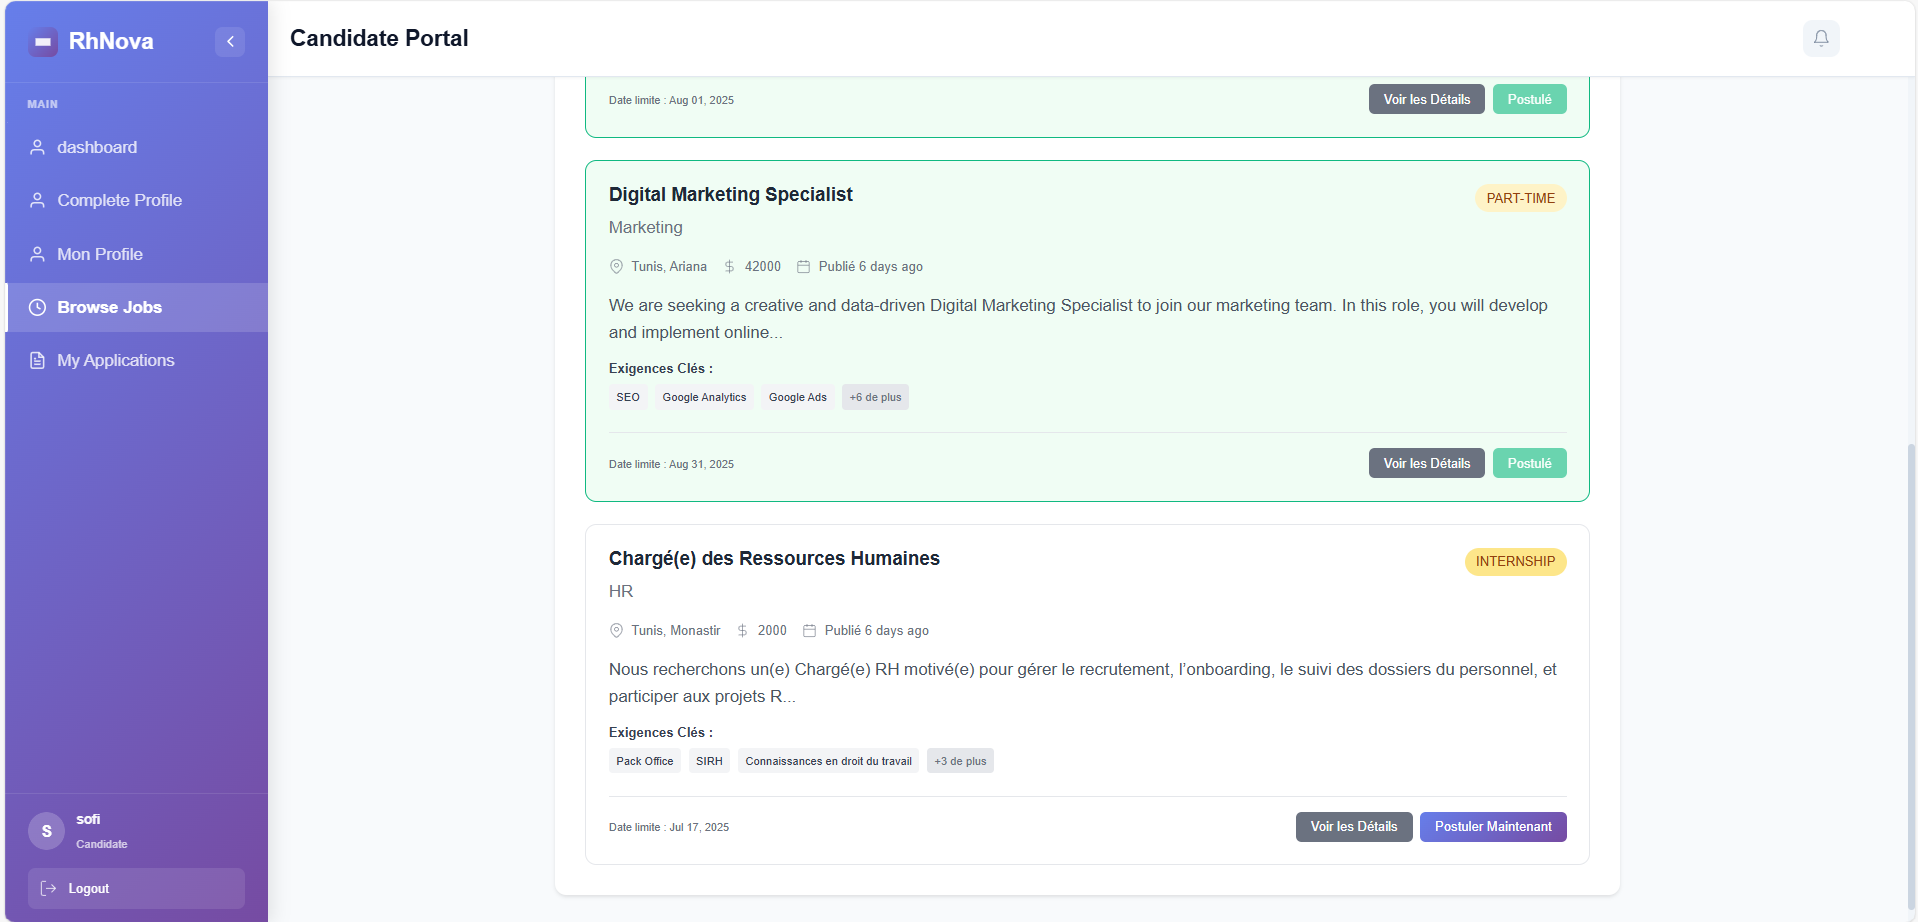
\includegraphics[width=\textwidth]{Figures/candidatoffre.png}
             \caption{Liste des offres}
         \end{figure}
\end{itemize}
\begin{itemize}
     \item\textbf{Suivi des candidatures : }
Cette interface permet au candidat de suivre l’avancement de ses candidatures. Il peut consulter le statut de chaque étape du processus (soumission, entretien, décision finale) et accéder aux détails de ses entretiens, y compris la date, l’heure et le type d’entretien, ainsi qu’un lien vers l’enregistrement si disponible.
         \begin{figure}[H]
             \centering
             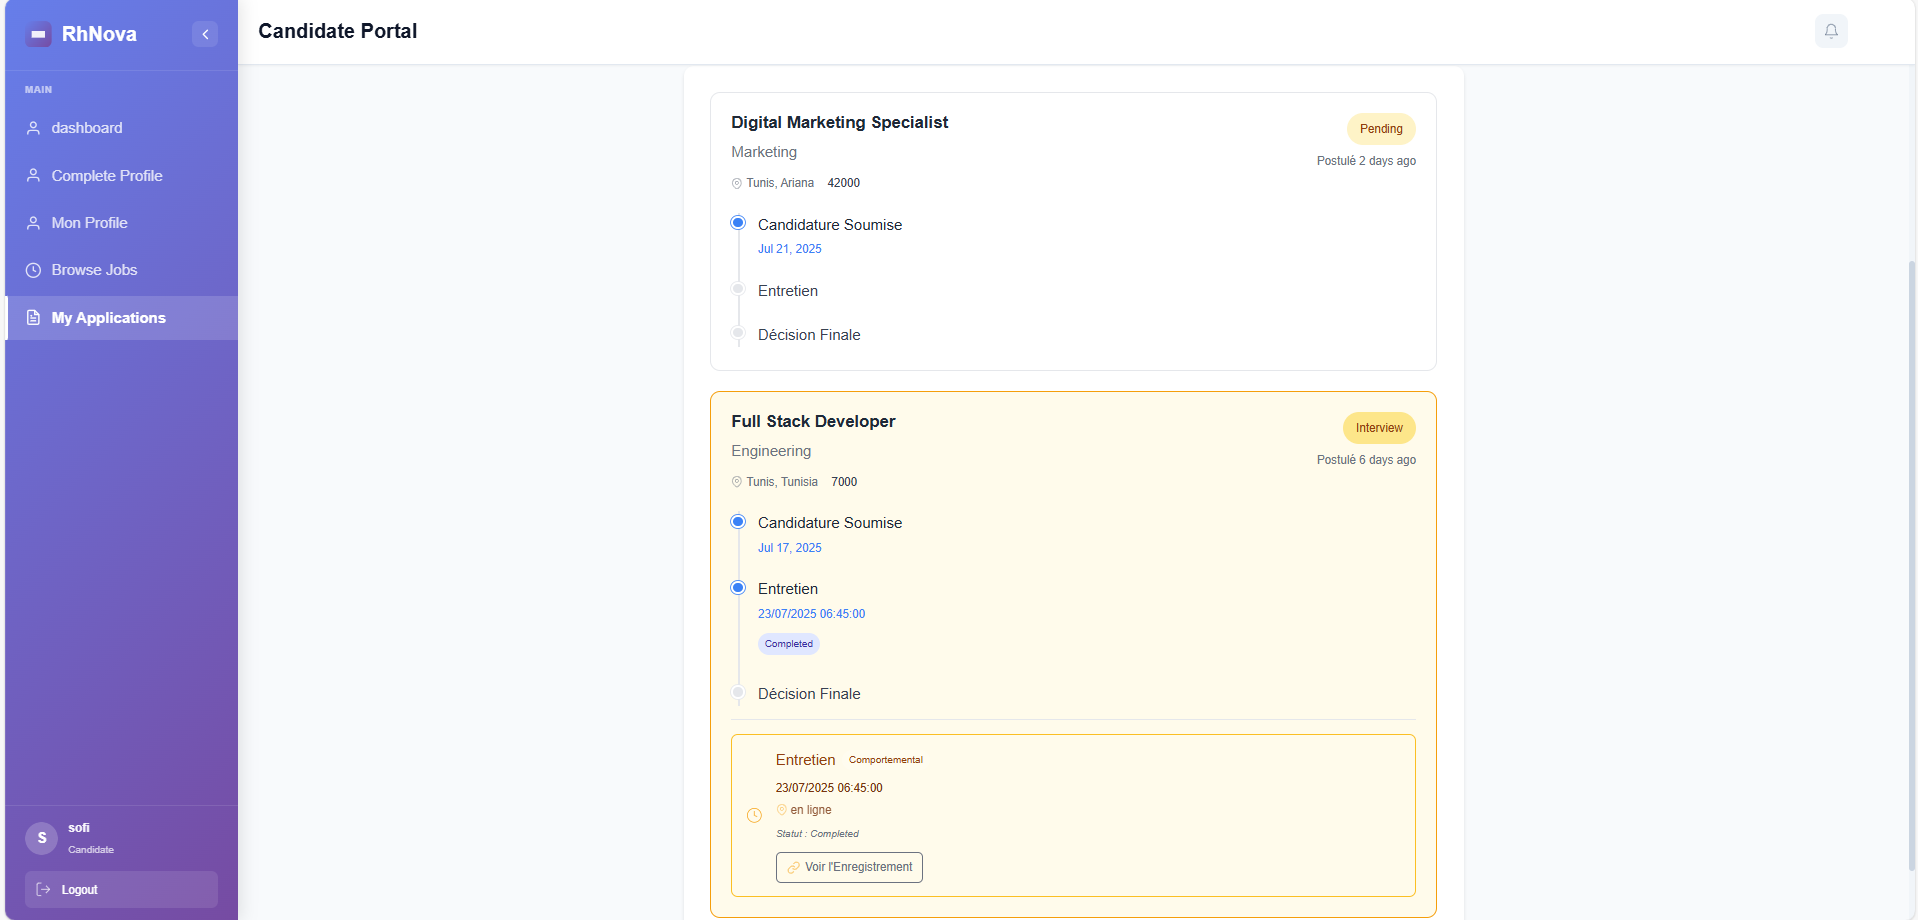
\includegraphics[width=\textwidth]{Figures/candidatsuivre.png}
             \caption{Suivi des candidatures}
         \end{figure}
     \end{itemize}

\section*{Conclusion}
En conclusion, ce chapitre a encadré la Sprint Gestion de Recrutement et Candidatures, en établissant les objectifs et détaillant le backlog, tout en exposant les diagrammes de cas d’utilisation, classes et de séquences. Les descriptions textuelles et captures d’écran ont confirmé la mise en œuvre réussie, posant des fondations robustes pour les phases de recrutement futures.Dans le chapitre suivant, nous aborderons les détails du troisième sprint " Gestion des Entretiens et ATS".
\addcontentsline{toc}{section}{\protect\numberline{}Conclusion}%




 